\chapter{Programming using Bootloader}

\emph{Bootloader} is a short program used to burn the firmware to the microcontroller without any programmer device. It is the first thing to run on device power on and is accessible through the serial interface.

\section{USB connection (obsolete)}

Setup described in this section enables you to program Main Boards using wired connection (i.e. mini USB cable) Bootloader.

\subsection{Programming the Bootloader on Main Board}
\label{subsec:programming_the_bootloader}

A prerequisite to using Bootloader to program the Main Board is having the Bootloader itself configured and programmed onto the board. USB (wired) Bootloader is provided in \texttt{UART\_BOOTLOADER} project of PSoC creator \texttt{MU31S-000} workspace.

Steps:
\begin{enumerate}
	\item Build the project (right click on project name > Build \texttt{UART\_BOOTLOADER}).
	\item Set \texttt{UART\_BOOTLOADER} project to active (right click on project name > Set As Active Project).
	\item Connect MiniProg to MB and the PC.
	\item Program the MB (\textit{program} button in PSoC creator or Ctrl+F5).
	\item If asked, select a device to program. Sometimes the connection between MB and MiniProg is bad so make sure you adjust the cable until the device \texttt{PSoC 5LP CY8C5888LTI*-LP097} is detected. %TODO version??
	\item Once the device is detected, select \texttt{Port Acquire} > \texttt{Connect} > \texttt{OK} and wait for the completion of programming process.
\end{enumerate}

\subsection{Programming MB using Bootloader}
\label{subsec:programming_with_bootloader}

In order to program Main Board using Bootloader, \texttt{Bootloadable} component on MB has to be running and awaiting for programming request. It can be achieved by setting a waiting time after each system power on during which MB enters this mode. It is, however, not efficient because we sometimes need to program MB without power cycling it. Therefore, programs devised for Main Board always need to have one \textit{interpreter} task running which activates Bootloadable on request. This mode is entered by sending \texttt{'b'} character to MB's general purpose (debugging) UART.

\begin{figure}[htb]
    \centering
	  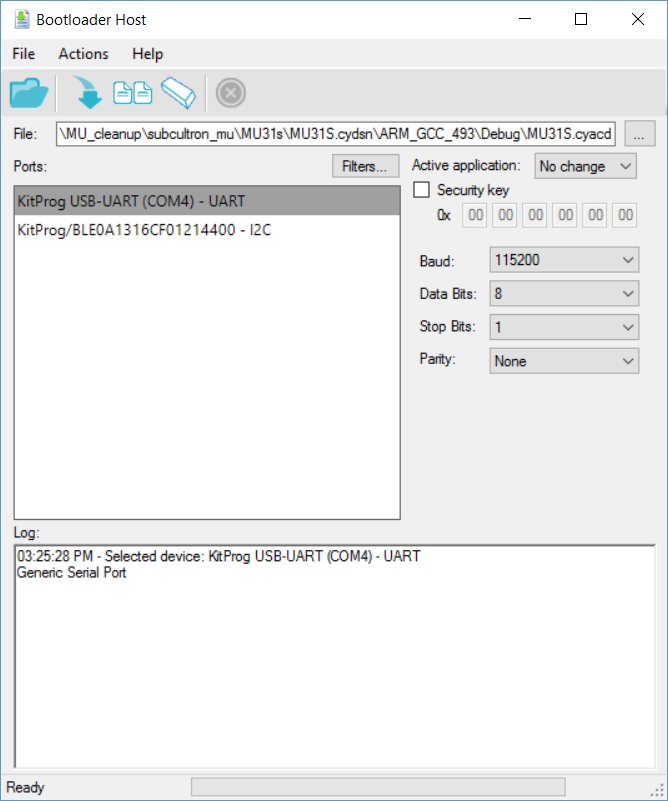
\includegraphics[width=0.6\linewidth]{figures/Bootloader_BLE.png}
	\caption{Setting up Bootloader Host}
	\label{fig:bootloader_host}
\end{figure}

The next step is to connect to the Main Board and start the programming process.\\
Steps:
\begin{enumerate}
	\item Connect the MB to your PC via mini USB cable. Make sure all connections to this COM port are closed (stop connections in Docklight).
	\item Open the project you wish to program in PSoC Creator.
	\item Go to \texttt{Tools} > \texttt{Bootloader Host}.
	\item Select the correct COM port and adjust settings to match the ones in Figure \ref{fig:bootloader_host}.
	\item Click on \texttt{Program} button and wait for the process to execute.
\end{enumerate}

\section{BLE Bootloader}

The process of programming MB using BLE Bootloader is the same as the one using wired connection Bootloader. The only difference is in the way the connection to the device is established (step 1 in the previous section). For guide on setting up BLE bridge between MB and PC, refer to Chapter \ref{ch:connecting_to_ble}. Bootloader project that needs to be programmed onto the Main Board is \texttt{UART\_Bootloader\_BLE}.

\section{I2C Bootloader}

...